\documentclass[UTF8]{ctexart}
% 基本设置和必要宏包
\usepackage{geometry}
\geometry{a4paper,scale=0.8}

% 数学相关宏包
\usepackage{amsmath}
\usepackage{amssymb}
\usepackage{amsfonts}

\usepackage{mathtools}
\usepackage{amsbsy}
\usepackage{amstext}
\usepackage{wasysym}
\usepackage{stmaryrd}
\usepackage{mathrsfs}

% 图形和颜色
%\usepackage{xcolor}
\usepackage{graphicx}
\usepackage{subcaption}
\usepackage{caption}
\usepackage{float}


% 其他功能性宏包
\usepackage{titlesec}
\usepackage{fancyhdr}
\usepackage{setspace}
\usepackage{cite}
\usepackage{appendix}
\usepackage{listings}
\usepackage{pdfpages}
\usepackage{enumitem}
\usepackage{tabu}
\usepackage{threeparttable}
\usepackage{booktabs}
\usepackage{abstract}
\usepackage{multirow}


\usepackage{diagbox} 

% 允许公式跨页
\allowdisplaybreaks[4]



\newcommand{\sihaoheiti}{\fontsize{14pt}\selectfont\heiti}
% 设置全局字体
%\setCJKmainfont{SimSun} % 设置正文为宋体
%\setCJKsansfont{SimHei} % 设置无衬线字体为黑体

% 论文题目设置为三号黑体字,并居中
\newcommand{\threelargebf}{\fontsize{16pt}{19.2pt}\selectfont\heiti\centering}

% 一级标题设置为四号黑体字,并居中
\titleformat{\section}{\centering\fontsize{14pt}{16pt}\bfseries\heiti}{\thesection}{1em}{}

% 二级标题设置为小四号黑体字,左对齐
\titleformat{\subsection}{\fontsize{12pt}{14.4pt}\bfseries\heiti}{\thesubsection}{1em}{\raggedright}

% 三级标题设置为小四号黑体字,左对齐
\titleformat{\subsubsection}{\fontsize{12pt}{14.4pt}\bfseries\heiti}{\thesubsubsection}{1em}{\raggedright}

% 正文字体设置为小四号宋体字,并使用单倍行距
\renewcommand{\normalsize}{\fontsize{12pt}{14.4pt}\selectfont}
%\renewcommand{\baselinestretch}{3}
%\selectfont



%\linespread{5.0}%修改行距
% 图片文件夹
\graphicspath{{img/}}

\let\itemize\compactitem
\let\enditemize\endcompactitem

% 设置页面布局
\geometry{a4paper, left=2.5cm, right=2.5cm, top=3cm, bottom=3cm}
\setstretch{1.2}

\renewcommand{\arraystretch}{1.5}
\newcommand{\thickhline}{\noalign{\hrule height 1.2pt}} % 设置粗线的宽度
\newcommand{\thinhline}{\noalign{\hrule height 0.8pt}} % 设置细线的宽度

%%%% ===== 定理环境
\usepackage[amsmath,thref,thmmarks,hyperref]{ntheorem} % 定理宏包
%\theorempreskipamount1em % spacing before the environment
%\theorempostskipamount0em  % spacing after the environment
%\theoremstyle{plain}
%\theoremheaderfont{\normalfont\heiti}
%\theorembodyfont{\normalfont\kaishu}
%\theoremindent0em
%\theoremseparator{\hspace{0.2em}}
%\theoremnumbering{arabic}

\newtheorem{property}{性质}[section]
\newtheorem{definition}{定义}[section]
\newtheorem{lemma}{引理}[section]
\newtheorem{remark}{注记}[section]
\newtheorem{corollary}{推论}[section]
\newtheorem{example}{例}[section] 
\newtheorem{problem}{{问题}}

 \renewcommand{\abstractnamefont}{\normalfont\bfseries}  % 摘要标题字体:正常字体,粗体
\renewcommand{\abstracttextfont}{\normalfont\normalsize}     % 摘要内容字体:正常字体,小四号

% 设置页眉页脚
\pagestyle{fancy}
\fancyhf{}
\fancyfoot[C]{\thepage}
\renewcommand{\headrulewidth}{0pt}

% 设置标题格式
\titleformat{\section}{\centering\heiti\large}{\thesection}{1em}{}
\titleformat{\subsection}{\raggedright\heiti\normalsize}{\thesubsection}{1em}{}
\titleformat{\subsubsection}{\raggedright\heiti\normalsize}{\thesubsubsection}{1em}{}

% 设置摘要环境
%\newenvironment{myabstract}{
%	\begin{center}
%	\bfseries\zihao{-3} 摘要
%	\end{center}
%	\vspace{-0.5em} % 调整摘要与论文题目的距离
%	\normalsize
%}{
%}
% 设置附录环境
\renewcommand{\appendixname}{附录}
\renewcommand{\appendixpagename}{附录}

% 设置代码环境
\lstset{
	basicstyle=\small\ttfamily,
	keywordstyle=\color{blue},
	commentstyle=\color{green!70!black},
	stringstyle=\color{red},
	breaklines=true,
	numbers=left,
	numberstyle=\tiny,
	frame=tb,
	language=Python
}
\newcommand{\bbA}{\mathbb{A}}
\newcommand{\bbB}{\mathbb{B}}
\newcommand{\bbC}{\mathbb{C}}
\newcommand{\bbD}{\mathbb{D}}
\newcommand{\bbE}{\mathbb{E}}
\newcommand{\bbF}{\mathbb{F}}
\newcommand{\bbG}{\mathbb{G}}
\newcommand{\bbH}{\mathbb{H}}
\newcommand{\bbI}{\mathbb{I}}
\newcommand{\bbJ}{\mathbb{J}}
\newcommand{\bbK}{\mathbb{K}}
\newcommand{\bbL}{\mathbb{L}}
\newcommand{\bbM}{\mathbb{M}}
\newcommand{\bbN}{\mathbb{N}}
\newcommand{\bbO}{\mathbb{O}}
\newcommand{\bbP}{\mathbb{P}}
\newcommand{\bbQ}{\mathbb{Q}}
\newcommand{\bbR}{\mathbb{R}}
\newcommand{\bbS}{\mathbb{S}}
\newcommand{\bbT}{\mathbb{T}}
\newcommand{\bbU}{\mathbb{U}}
\newcommand{\bbV}{\mathbb{V}}
\newcommand{\bbW}{\mathbb{W}}
\newcommand{\bbX}{\mathbb{X}}
\newcommand{\bbY}{\mathbb{Y}}
\newcommand{\bbZ}{\mathbb{Z}}

\title{}
\author{}
\date{}

\begin{document}


\begin{titlepage}		
		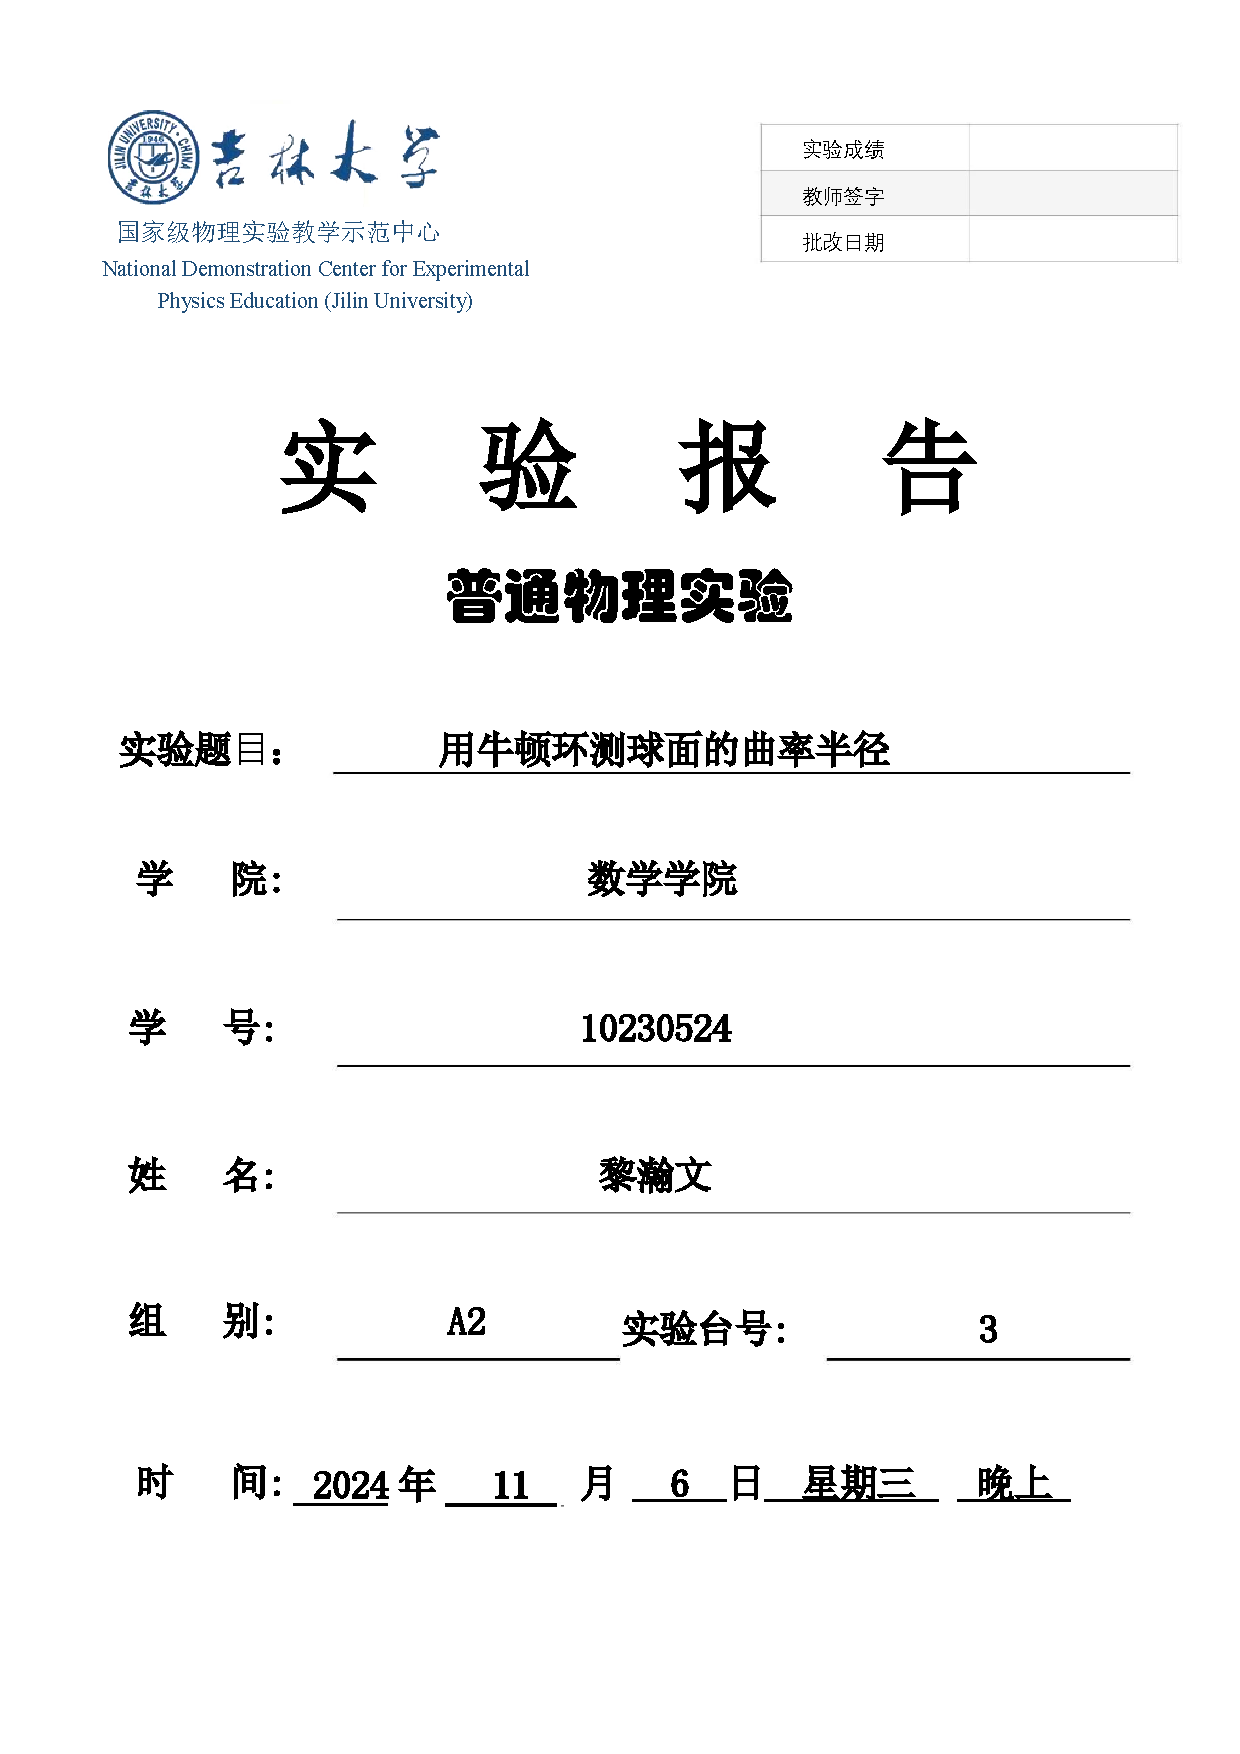
\includepdf[pages=-]{牛顿环封面.pdf}
\end{titlepage}


\section{实验原理}
凸透镜与平面玻璃板之间形成了空气薄膜,当波长为 $\lambda$ 的单色光垂直投射到装置上时,空气薄膜上下表面反射的光波会发生干涉。对于第 k 级暗环,其半径为$r^2_k = \frac{R\lambda}{n}k$。由于任意两干涉环的半径平方差和干涉环的顺序无关,只与两环的序数差有关。故 $R = \frac{r'^2_{k_{2}} - r'^2_{k_{1}}}{\lambda(k_2 - k_1)}$


\vspace{3cm} %5cm vertical space 绘制牛顿环原理图
\section{实验内容}
\begin{enumerate}
    \item 调节牛顿环仪的三个螺丝,使得形成的干涉纹位于正中心
    \item 打开钠光灯并预热约15分钟
    \item 将牛顿环仪放置在显微工作台上并使其中心对准显微镜筒的光轴
    \item 调节目镜使得看到的叉丝最清晰,并调整其角度使竖叉丝与镜筒走向垂直。
    \item 在离中心左侧第5环处记录读数$L'_5$,往环中心方向连续移动并记录另一侧第5环位置$L_5$和第25环位置$L_{25}$。随后反向移动并记录离中心第5环位置$L_5$,越过中心后的第5环位置$L'_5$和第25环位置$L'_{25}$。重复上述操作记录五组数据
    \item 计算和的标准差,以及相关量的不确定度
\end{enumerate}



\section{注意事项}
\begin{enumerate}
    \item 注意实验前钠灯预热15min;因为其含汞,所以不要摔倒地上;实验后注意关闭钠灯。
    \item 注意调节牛顿环螺丝时不要拧得过紧或过松
    \item 避免长时间查看,以免损坏眼睛
    \item 只能从下往上移动镜筒,从旁边观察以避免镜筒压到牛顿环
    \item 注意在实验过程测量一个方向数据时读数显微镜叉丝单向移动,以避免回程差
\end{enumerate}
\newpage
\section{原始数据}


\begin{table}[H]
    \caption{测量数据(单位:mm)}
    \begin{tabular}{|c|c|c|c|c|c|c|c|c|c|c|}
    \toprule[1pt]
       组别  &   $L'_5$  & $L_5$  &  $L_{25}$  &  $r_{k_2}+r_{k_1}$ & $r_{k_2}-r_{k_1}$ & $L_5$ & $L'_5$  &$L'_{25}$  & $r_{k'_2} + r_{k'_1} $ & $r_{k'_2} - r_{k'_1} $\\
    \midrule
       1  &  15.727 &11.301  & 8.661  & 7.066  & 2.640  &11.382  & 15.789  & 18.475  & 7.093  & 2.686 \\
    \midrule
       2  & 15.720 &  11.312  & 8.657  & 7.063  & 2.655  &11.380  & 15.783  & 18.471  & 7.091  & 2.688\\
    \midrule
       3  & 15.715 &  11.309  & 8.661  & 7.054  & 2.648  &11.370  & 15.790  & 18.475  & 7.105  & 2.685 \\
    \midrule
       4 & 15.726 &  11.310  & 8.655  & 7.071  & 2.655  &11.357  & 15.791  & 18.478  & 7.121  & 2.687 \\
    \midrule
        5 & 15.722 &  11.303  & 8.657  & 7.065  & 2.646  & 11.369  & 15.782  & 18.485  & 7.116  & 2.703 \\
    \bottomrule[1pt]
    \end{tabular}
\end{table}


实验中读数显微镜的最小分度值为 $0.001mm$



\section{数据处理}

上述实验过程中环数之差为 $k_2 - k_1 = 20$, $k'_2 - k'_1 = 20$
得到平均值 

\begin{align*}
   \overline{r_{k_2} + r_{k_1}} &= \frac{\sum r_{k_2}+r_{k_1} + \sum r_{k'_2}+r_{k'_1}}{10} = 7.0845 \  mm   \\
   \overline{ r_{k_2}-r_{k_1} } &= \frac{\sum r_{k_2}-r_{k_1} + \sum r_{k'_2}-r_{k'_1}}{10} = 2.6693 \  mm 
\end{align*}
\begin{align*}
    R = \frac{r^2_{k_2} - r^2_{k_1}}{\lambda (k_2 - k_1) } \\
    R' = \frac{r'^2_{k_2} - r'^2_{k_1}}{\lambda (k'_2 - k'_1) } \\
\end{align*}
   带入上式表格中数据,且 $\lambda = 598.3 \ nm$得到
\begin{table}[H]
\centering 
    \caption{计算得到曲率半径数值}
    \begin{tabular}{|c|c|c|c|c|c|}
    \toprule[1pt]
    $R$ &   1582.7456 &  1591.0627 & 1584.8457 &  1592.8648 &  1586.1183 \\
    \midrule
    $R'$ &   1616.4770 &  1617.2245 & 1618.6089  &  1623.4623 &  1631.9827 \\
    \bottomrule[1pt]
    \end{tabular}
\end{table}
曲率半径均值$\overline{R}$为
\begin{align*}
    \overline{R} &= \frac{\sum_{i=1}^{5} R + \sum_{i=1}^{5} R'}{10}  \\
    &= \frac{1}{10} \times(1582.7456 +  1591.0627  + 1584.8457 +  1592.8648 +  1586.1183 + 1616.4770 +  1617.2245 + \\ 
    &1618.6089  +  1623.4623 +  1631.9827) \ mm  \\
    &= 1604.5393  \ mm 
\end{align*}
标准偏差 S(R) 为
\begin{align*}
    S(R) &= \sqrt{\frac{ \sum_{i=1}^{10} (R - \overline{R})^2}{10 \times (10 -1)}} \\
      &= 5.8998 \ mm
      \end{align*}
故求得上述牛顿环曲率半径为 $R = 1604.5393 \  mm $,标准偏差为 $S(R) = 5.8998 \ mm$

\textbf{A类测量不确定度的计算}

\begin{align*}
 u_A(r_{k_2} + r_{k_1}) &= \sqrt{ \frac{  \sum \Big(  (r_{k_2} + r_{k_1})  -   \overline{r_{k_2} + r_{k_1}}  \Big)^2 }{   10 * 9 }   }  = 0.0076 \ mm \\
u_A(r_{k_2} - r_{k_1}) &= \sqrt{ \frac{  \sum \Big(  (r_{k_2} - r_{k_1})  -   \overline{r_{k_2} - r_{k_1}}  \Big)^2 }{   10 * 9 }   }  = 0.0071 \ mm 
\end{align*}

\textbf{B类不确定度的计算} 

已知上述实验过程中读数显微镜的最小分度值为 $ \Delta = 0.01mm$,则测量任意环的位置时,假设误差均匀分布
\begin{align*}
    u_B(L_k) = u_B(L'_k) = \frac{\Delta}{\sqrt{3}} = \frac{0.01}{\sqrt{3}} \ mm = 0.0058 \ mm
\end{align*}
由不确定度传递公式
\begin{align*}
    u_B(r_{k_2} + r_{k_1}) &= \sqrt{u_B(k_2)^2 + u_B(k_1)^2 } = \sqrt{0.0058^2 + 0.0058^2} \ mm = 0.0082 \ mm \\
     u_B(r_{k_2} - r_{k_1}) &= \sqrt{u_B(k_2)^2 + u_B(k_1)^2 } = \sqrt{0.0058^2 + 0.0058^2} \ mm = 0.0082 \ mm
\end{align*}


\textbf{合成不确定度的计算}

\begin{align*}
    u_c(r_{k_2} + r_{k_1}) &= \sqrt{u^2_A(r_{k_2} + r_{k_1}) + u^2_B(r_{k_2} + r_{k_1})} = \sqrt{ 0.0076^2 + 0.0082^2}  \ mm = 0.0112 \ mm \\
    u_c(r_{k_2} - r_{k_1}) &= \sqrt{u^2_A(r_{k_2} - r_{k_1}) + u^2_B(r_{k_2} - r_{k_1})} = \sqrt{ 0.0071^2 + 0.0082^2}  \ mm = 0.0108 \ mm
\end{align*}

由标准的不确定度传递公式 
\begin{align*}
    y &= f(x_1,x_2,\dots,x_n) \\
    u_c(y) &= \sqrt{\sum_{i=1}^{n}(\frac{\partial f}{\partial x_i})^2 u^2_{c(x_i)}}
\end{align*}
结合 $R = \frac{r^2_{k_2} - r^2_{k_1}}{\lambda (k_2 - k_1) }$
得到
\begin{align*}
    u_R &= \sqrt{ \Big(\frac{\partial R}{\partial (r_{k_2} + r_{k_1})} \Big)^2 u^2_c(r_{k_2} + r_{k_1})  + \Big(\frac{\partial R}{\partial (r_{k_2} - r_{k_1})} \Big)^2 u^2_c(r_{k_2} - r_{k_1})  } \\
    \frac{u_R}{R} &=  \sqrt{  \Big( \frac{u_c(r_{k_2} + r_{k_1})}{\overline{r_{k_2} + r_{k_1}}}  \Big)^2 + \Big( \frac{u_c(r_{k_2} - r_{k_1})}{\overline{r_{k_2} - r_{k_1}}}  \Big)^2  }
\end{align*}
带入 $R = 1604.5393 \ mm$、$ u_c(r_{k_2} + r_{k_1}) = 0.0112 \ mm$、$ u_c(r_{k_2} - r_{k_1}) = 0.0108 \ mm$、$\overline{r_{k_2} + r_{k_1}} = 7.0845 \ mm$、$\overline{r_{k_2} - r_{k_1}} = 2.6693 \ mm$可得
\begin{align*}
    u_R &= \sqrt{  \Big( \frac{0.0112}{7.0845}  \Big)^2 + \Big( \frac{0.0108}{2.6693} \Big)^2  } \times 1604.5393 \ mm \\
    u_R &= 6.9700 \ mm
\end{align*}
由 $p=0.955$,对应的置信概率 $K_p=2$。代入上述数据及公式 $U_i = K_p \times u_i$ 可得其扩展不确定度如下:
\begin{align*}
    U_R = K_p \times u_R = 2 \times 6.9700 \ mm = 13.9400 \ mm 
\end{align*}
故得到 曲率半径 $R = 1604.5393 \pm 13.9400 \ mm $,$p = 0.955$
\section{拓展实验}
\subsection{将钠光灯替换为手机手电筒的白光光源,观察到的现象}
观察到明暗相间的彩色圆环。

原因:白光是由多种色光混合而成,且波长各不相同,每种单色光独立发生干涉,最终形成了彩色的圆环


\subsection{移除半反镜,组成投射式牛顿环,观察到的现象与之前有何不同}
中心从暗斑变成亮斑;亮斑与暗斑的亮度差异下降了,同心圆环不如之前清晰,但仍然存在;新的同心圆环的亮暗交替,并且与原来相比暗纹变为亮纹,亮纹变为暗纹


\vspace{7cm}

\section{思考题}
\subsection{牛顿环干涉条纹形成的两个反射表面以及产生条件}
牛顿环形成的干涉条纹发生在凸透镜凸表面和玻璃板的平面,其干涉条纹由光线在这两个面之间反射形成。产生的条件是两束光振动方向相同、波长相同、相位差恒定且能够在空间中相遇

\subsection{牛顿环干涉条纹的中心暗亮的情况}
干涉形成的牛顿环,其中心的亮暗取决于透镜和平面玻璃板所夹介质的折射率。当介质的折射率小于玻璃的折射率时,由于半波损失,形成暗斑。当介质的折射率大于玻璃的折射率时,形成亮斑。并且在透射情形下,光经过玻璃板上表面与透镜下表面后发生相长干涉,从而形成亮斑

\subsection{干涉条纹相邻暗(亮)环之间的距离分析}
在越靠近中心的位置,相邻暗(亮)环之间的距离越大;越远离中心,相邻暗(亮)环之间的距离越小

\subsection{为什么说测量显微镜测量的是牛顿环的直径,而不是显微镜内被放大了的直径?改变显微镜的放大倍率是否会影响测量结果}
因为读数时并不是通过显微镜,而是在外面读取镜筒所处的位置。放大只是为了更加准确的确定镜筒所应该停在的位置。改变倍率不会改变测量结果,但是提高放大倍率能够提高测量的精确度

\subsection{如何用等厚干涉原理检验光学平面的表面质量}
用等厚干涉原理检验光学平面的表面质量时,如果表面质量良好,发生干涉后呈现的现象会是规则的明暗相间的同心圆环;如果表面质量不好,则发生干涉后呈现的明暗条纹会在特定位置发生不规则的弯曲,无法形成规整的同心圆。发生不规则弯曲的位置即为质量出现问题的位置
\end{document}